%\usepackage{amsmath, amssymb, ../../vimacros, hyperref, tikz}
%\usetikzlibrary{positioning, fit, bayesnet, shapes.misc, patterns}
%\usepackage{mathalfa}
%\usepackage{cancel}



\section{Reparameterised Gradient}

\begin{frame}{Change of density}

	For Gaussians
	\only<1>{
	\begin{equation*}
		\begin{aligned}
			z &\sim \mathcal N(\mu, \sigma^2) 
			\qquad &\frac{z - \mu}{\sigma^2} &\sim \mathcal N(0, 1)
		\end{aligned}
	\end{equation*}
	}
	\only<2->{
	\begin{equation*}
		\begin{aligned}
			z &\sim \mathcal N(\underbrace{\mu, \sigma^2}_{\alert{\lambda}}) 
			\qquad &\underbrace{\frac{z - \mu}{\sigma^2}}_{\alert{\epsilon = \inv{t}(z, \lambda)}} &\sim \mathcal N(0, 1)
		\end{aligned}
	\end{equation*}
	}
	
	\pause
	
	More generally
	\begin{equation*}
		\begin{aligned}
		f_{Z|\lambda}(z) &= s(\underbrace{\inv{t}(z, \lambda)}_{\epsilon }) \djac{\inv{t}}{z, \lambda}  \\ \pause
		\mathbb E_{f_{Z|\lambda}(z)}\left[ \psi(z) \right] &= \pause \underbrace{\mathbb E_{s(\epsilon)}\left[ \psi(t(\epsilon, \lambda) \right]}_{\text{\textcolor{blue}{check class on ADVI}}}
		\end{aligned}
	\end{equation*}
\end{frame}

\begin{frame}{Reparameterised gradient}

	\begin{equation*}
		\begin{aligned}		
		\pdv{\lambda}\mathbb E_{f_{Z|\lambda}(z)}\left[ \psi(z) \right] &= \mathbb E_{s(\epsilon)}\left[ \pdv{\lambda} \psi(t(\epsilon, \lambda) \right] \\ \pause
		&= \mathbb E_{s(\epsilon)}\left[ \pdv{z} \psi(z) \pdv{\lambda}  t(\epsilon, \lambda) \right] 
		\end{aligned}
	\end{equation*}
	
	Easy to MC estimate!

	
\end{frame}

\begin{frame}{Comparing gradient estimators}

	Reparameterised gradient\hfill Score function estimator
	\begin{equation*}
		\mathbb E_{s(\epsilon)}\left[ \underbrace{\pdv{z} \psi(z) \pdv{\lambda} t(\epsilon, \lambda)}_{\hat g_{\text{rep}}} \right]  ~ = ~ \mathbb E_{f_{\lambda}(z)}\left[\underbrace{\psi(z) \pdv{\lambda} f_{Z|\lambda}(z)}_{\hat g_{\text{sfe}}} \right]
	\end{equation*}
	
	
	\begin{itemize}

		\item $\hat g_{\text{sfe}}$ is typically cursed with variance
		\item but is $\hat g_{\text{rep}}$ available in general? \\ \pause
		 in particular, is it available for discrete variables?
	\end{itemize}
\end{frame}

\begin{frame}{A general reparameterisation}

	What transformation will always absorb the parameters of a density? \pause
	\begin{equation*}
		\begin{aligned}
			Z &\sim f_{Z|\lambda}(z) \\
			F_{Z|\lambda}(z) &\sim \mathcal U(0, 1)			
		\end{aligned}
	\end{equation*}
	
	\pause
	
	So, if I know the inverse cdf, 
	\begin{equation*}
		\begin{aligned}
		\epsilon &\sim \mathcal U(0, 1) \\
		z &= \inv{F}_{Z|\lambda}(\epsilon) 
		\end{aligned}
	\end{equation*}
	do I have access to $\hat g_{\text{rep}}$?
\end{frame}



\begin{frame}{Let's reparameterise a Bernoulli}

	\begin{columns}
	\begin{column}{0.35\textwidth}
	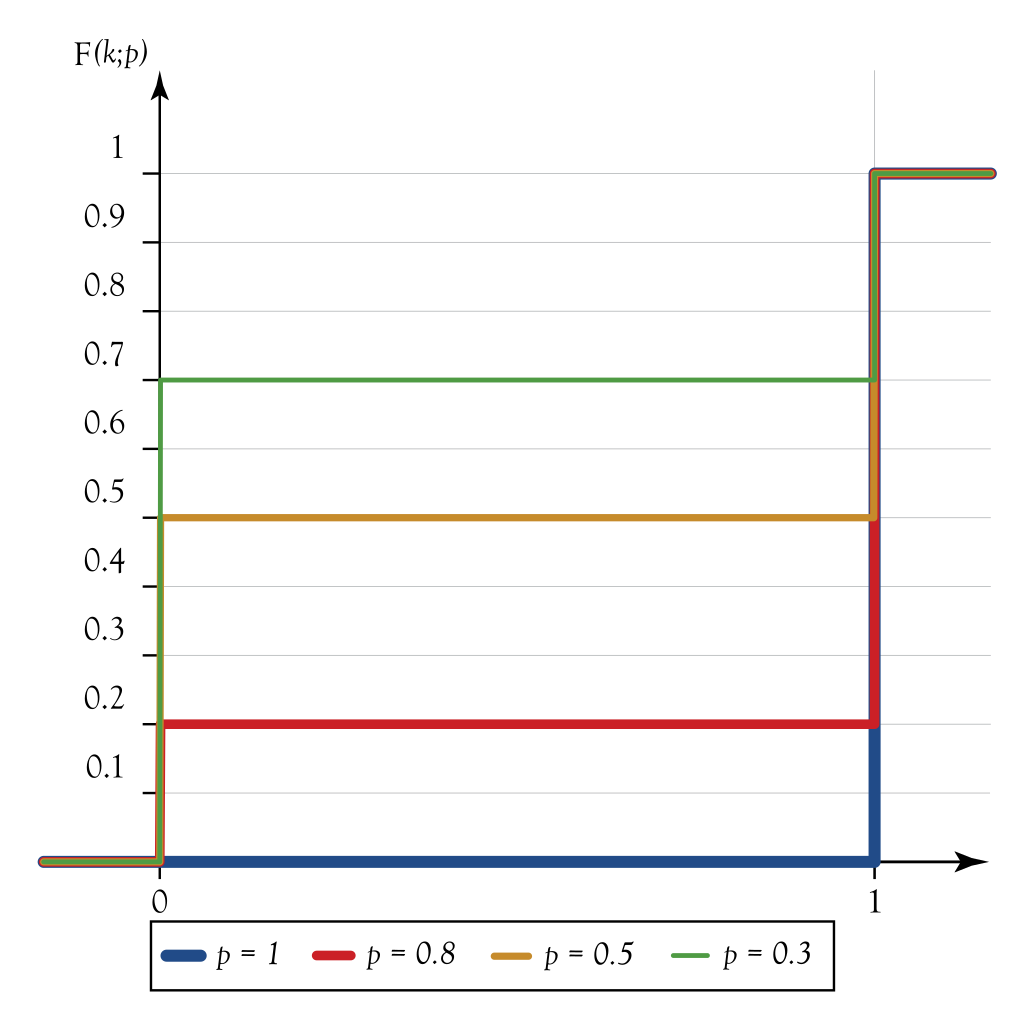
\includegraphics[scale=0.15]{bernoulli-cdf}
	\end{column}
	~
	\begin{column}{0.45\textwidth}
	\begin{equation*}
		\begin{aligned}
			Z &\sim \Bernoulli(p) \\ \pause
			\inv{F}_{Z|p}(\epsilon) &= 
			\begin{cases}
			0 &\text{if }\epsilon < 1 - p \\
			1 &\text{otherwise}
			\end{cases}
		\end{aligned}
	\end{equation*}
	\end{column}

	\end{columns}
	
	~
	
	\pause
	
	How about $\pdv{p}\inv{F}_{Z|p}(\epsilon)$? \pause \alert{Mostly $0$, sometimes undefined!}
	
\end{frame}

\begin{frame}{Discrete case}
	Discrete variables do not admit a differentiable reparameterisation. The cells of the Jacobian are either $0$ or undefined :/
	
	~ \pause
	
	The score function estimator is fully general, but very noisy.
	
	~ \pause
	
	Ask the deep learning literature for help :D \\ \pause
	~ \alert{Fake a Jacobian!}
\end{frame}

\section{Biased Gradient Estimates for Discrete Variables}


\begin{frame}{Straight-Through Estimator (STE)}

	In lack of a Jacobian, use the identity
	\begin{equation*}
		\jac{\inv{t}}{\epsilon, \lambda} = \diag(\mathbf 1)
	\end{equation*}
	
	
	STE is a biased gradient estimator that works in some cases, but unfortunately there are no general recipes.
	
\end{frame}

\begin{frame}{Bernoulli-STE}

	Consider a VAE where $q(z|x) = \Bern(z|g(x; \lambda))$. \pause \\
	We sample $z$ via a reparameterisation that absorbs $\lambda$:
	\begin{equation*}
		\begin{aligned}
			\epsilon \sim \mathcal U(0, 1) & \quad & p = g(x; \lambda) & \quad & z= \underbrace{\mathds 1_{(0, p)}(\epsilon)}_{t} 
		\end{aligned}
	\end{equation*}
	\pause
	A gradient estimate of the ELBO involves computing:
	\begin{equation*}
		\pdv{\lambda} \log p(x|z=t(\epsilon, \lambda)) = \pdv{z} \log p(x|z) \alert{\pdv{\lambda} t(\epsilon, \lambda)}
	\end{equation*}	
	\pause
	and we use our \emph{pseudo gradient}
	\vspace{-10pt}
	\begin{equation*}
		\begin{aligned}			
			\pdv{\lambda} t(\epsilon, \lambda) &=  \pdv{\lambda} g(x; \lambda)\cancelto{\overset{\text{def}}{=}1}{\alert{ \pdv{p} \mathds 1_{(0, p)}(\epsilon)}} 
		\end{aligned}
	\end{equation*}
	
	%Think of it as ignoring the discontinuities introduced by $t$

\end{frame}


\begin{frame}{Concrete (Gumbel-Softmax) Distribution}

	We can sample from a Categorical distribution via
	\begin{equation*}
	\begin{aligned}
		\epsilon_k &\sim \Gumbel(0, 1) \\
		\underbrace{\argmax_k ~ \{\lambda_k + \epsilon_k\}_{k=1}^K }_{z=t(\epsilon, \lambda)} &\sim \Cat(\softmax(\lambda)) \\		
	\end{aligned}
	\end{equation*}
	
	\pause
	
	The problem is that $t(\epsilon, \lambda)$ is not differentiable, but note 	
	\begin{equation*}
		\onehot(z) \approx \softmax\left(\frac{\lambda + \epsilon}{\tau}\right)  \qquad \text{as } \tau \to 0
	\end{equation*}
	and now the transformation is differentiable, but the outcome is dense. For sparsity, use (biased) STE.
	
	
\end{frame}

\begin{frame}{Summary}

	\begin{itemize}
		\item The inverse cdf is a general reparameterisation procedure
		\item In the discrete case, its inverse is piecewise constant
		\item Relaxations of Categorical variables are based on the idea of relaxing the one-hot representation of the outcome
		\item Dense relaxations are mapped to sparse (one-hot) representations via a discontinuity which is ignored in backpropagation (STE).
	\end{itemize}
\end{frame}

\nocite{bengio2013estimating}
\nocite{MaddisonEtAl2017:Concrete}
\nocite{JangEtAl2017:GumbelSoftmax}
\nocite{rolfe2016discrete}
\nocite{louizos2017learning}
\nocite{bastings-etal-2019-interpretable}

\begin{frame}[allowframebreaks]{Literature}
%\bibliographystyle{plainnat}
\bibliographystyle{unsrtnat}
\bibliography{../../VI}
\end{frame}
